\documentclass[12pt,UTF8]{ctexbook}

% 设置纸张信息
\input{../../../../common/page}

% 设置字体
\xeCJKsetup{AutoFallBack=true}
\setCJKfamilyfont{hei}{SimHei}
\setCJKfamilyfont{kai}{KaiTi}

% 目录 chapter 级别加点（.）
\usepackage{titletoc}
\titlecontents{chapter}[0pt]{\vspace{3mm}\bf\addvspace{2pt}\filright}{\contentspush{\thecontentslabel\hspace{0.8em}}}{}{\titlerule*[8pt]{.}\contentspage}

% 设置 part 和 chapter 标题格式
\ctexset{
	part/name= {第,卷},
	part/number={\chinese{part}},
	chapter/name={第,篇},
	chapter/number={\arabic{chapter}}
}

% 图片相关设置
\usepackage{graphicx}
\graphicspath{{Images/}}

% 列表项向右偏移
\usepackage{enumitem}
% 强制表格位置
\usepackage{float}
% 数学公式支持
\usepackage{amsmath}
\usepackage{amssymb}

\title{\heiti\zihao{0} 电容}
\author{WangFei}
\date{\today}

\begin{document}

\maketitle
\tableofcontents

\frontmatter
\chapter{前言}

电容是收音机等电子设备中不可或缺的重要电子元件，本章节将详细介绍电容的基本特性、分类、应用以及选择原则等内容。

\mainmatter

% 增加空行
~\\

\chapter{电容的基本概念}

\section{电容的基本原理}

\subsection{电容的定义}

\subsection{电容的结构}

\subsection{电容的主要参数}

\section{电容的工作原理}

\subsection{充电过程}

\subsection{放电过程}

\subsection{电容的储能}

\chapter{电容的分类}

\section{按介质分类}

\subsection{陶瓷电容}

\subsubsection{瓷片电容}

\subsubsection{独石电容}

\subsubsection{MLCC（多层陶瓷电容）}

\subsubsection{安规陶瓷电容}

\subsection{电解电容}

\subsubsection{铝电解电容}

\subsubsection{固态电容}

\subsubsection{钽电容}

\subsection{薄膜电容}

\subsubsection{CBB电容（聚丙烯电容）}

\subsubsection{涤纶电容（聚酯电容）}

\subsubsection{聚苯乙烯电容}

\subsubsection{聚碳酸酯电容}

\subsection{云母电容}

\subsection{纸介电容}

\subsection{安规电容}

安规电容是指获得安全认证机构认证、符合安全标准的电容，广泛应用于需要满足安全要求的电子设备中，特别是电源输入电路。安规电容在故障情况下能够保证设备和人员的安全，是电子设备安全设计的重要组成部分。

\subsubsection{安规电容的基本概念}

安规电容的主要特点包括：

\begin{itemize}[leftmargin=2cm]
    \item \textbf{安全认证}：通过国际或国家安全认证机构认证
    \item \textbf{可靠性高}：具有高可靠性和长寿命
    \item \textbf{抗电涌能力强}：能够承受电压浪涌和脉冲
    \item \textbf{阻燃性能好}：在故障情况下不会燃烧或蔓延火焰
    \item \textbf{自愈能力}：某些类型具有自愈功能
\end{itemize}

\subsubsection{安规电容的安全标准}

主要的安规电容安全标准包括：

\begin{itemize}[leftmargin=2cm]
    \item \textbf{UL标准}：美国保险商实验室标准（UL 60384-14）
    \item \textbf{IEC标准}：国际电工委员会标准（IEC 60384-14）
    \item \textbf{EN标准}：欧洲标准（EN 60384-14）
    \item \textbf{GB标准}：中国国家标准（GB/T 14472）
    \item \textbf{CSA标准}：加拿大标准协会标准
    \item \textbf{VDE标准}：德国电气工程师协会标准
\end{itemize}

\subsubsection{安规电容的分类}

安规电容根据其在电路中的作用和连接方式，主要分为X电容和Y电容两大类。

\subsubsection{X电容}

X电容是跨接在交流电源相线（L）和零线（N）之间的安规电容，用于抑制差模干扰。

\begin{figure}[H]
    \centering
    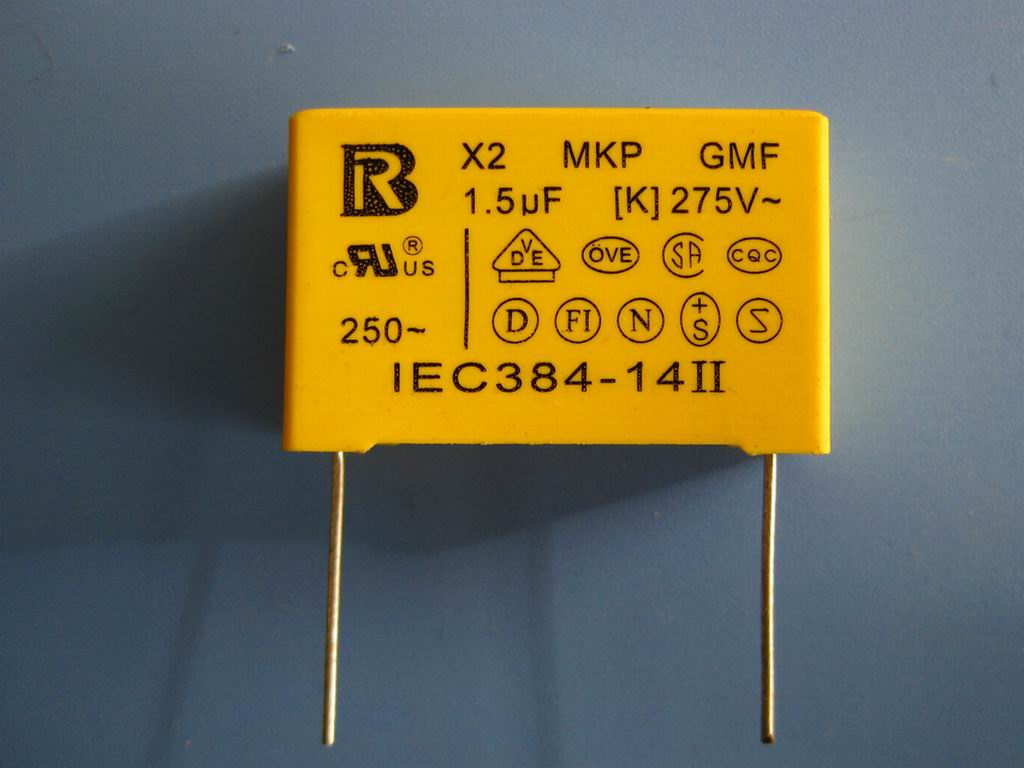
\includegraphics[width=0.6\textwidth]{安规电容X.jpg}
    \caption{X电容实物图}
    \label{fig:x_capacitor}
\end{figure}

\paragraph{X电容的作用}

X电容的主要作用包括：

\begin{itemize}[leftmargin=2cm]
    \item \textbf{抑制差模干扰}：滤除电源线上的差模噪声
    \item \textbf{EMI滤波}：作为EMI滤波器的重要组成部分
    \item \textbf{能量吸收}：吸收电压尖峰和浪涌
    \item \textbf{改善EMC性能}：提高设备的电磁兼容性
\end{itemize}

\paragraph{X电容的分类}

X电容根据其耐压等级可分为：

\begin{itemize}[leftmargin=2cm]
    \item \textbf{X1电容}：耐压 $\ge$ 2.5 kV，适用于高电压应用
    \item \textbf{X2电容}：耐压 $< 2.5$ kV 且 $\ge 1.2$ kV，最常用的类型
    \item \textbf{X3电容}：耐压 $< 1.2$ kV，适用于低电压应用
\end{itemize}

\paragraph{X电容的特点}

X电容的主要特点包括：

\begin{itemize}[leftmargin=2cm]
    \item \textbf{容值范围大}：通常为 0.01 $\sim$ 10 $\mu$F
    \item \textbf{耐压等级高}：能够承受高电压脉冲
    \item \textbf{自愈性能好}：故障后能够自动恢复
    \item \textbf{温度稳定性好}：在宽温度范围内性能稳定
    \item \textbf{使用寿命长}：设计寿命通常为10年以上
\end{itemize}

\paragraph{X电容的应用}

X电容的主要应用场景包括：

\begin{itemize}[leftmargin=2cm]
    \item \textbf{电源输入滤波}：AC-DC电源的输入端
    \item \textbf{开关电源}：各种开关电源的EMI滤波
    \item \textbf{家电设备}：电视机、冰箱、洗衣机等
    \item \textbf{工业设备}：工业控制设备、电机驱动等
    \item \textbf{通信设备}：路由器、交换机、服务器等
\end{itemize}

\paragraph{X电容的选择原则}

选择X电容时应考虑以下因素：

\begin{itemize}[leftmargin=2cm]
    \item \textbf{工作电压}：根据电源电压选择合适的X等级
    \item \textbf{容值大小}：根据滤波需求选择合适的容值
    \item \textbf{温度范围}：根据工作环境选择合适的温度等级
    \item \textbf{安全认证}：确保通过所需的安全认证
    \item \textbf{尺寸限制}：根据安装空间选择合适的封装
\end{itemize}

\subsubsection{Y电容}

Y电容是跨接在交流电源相线（L）与地线（PE）之间、零线（N）与地线（PE）之间的安规电容，用于抑制共模干扰。

\begin{figure}[H]
    \centering
    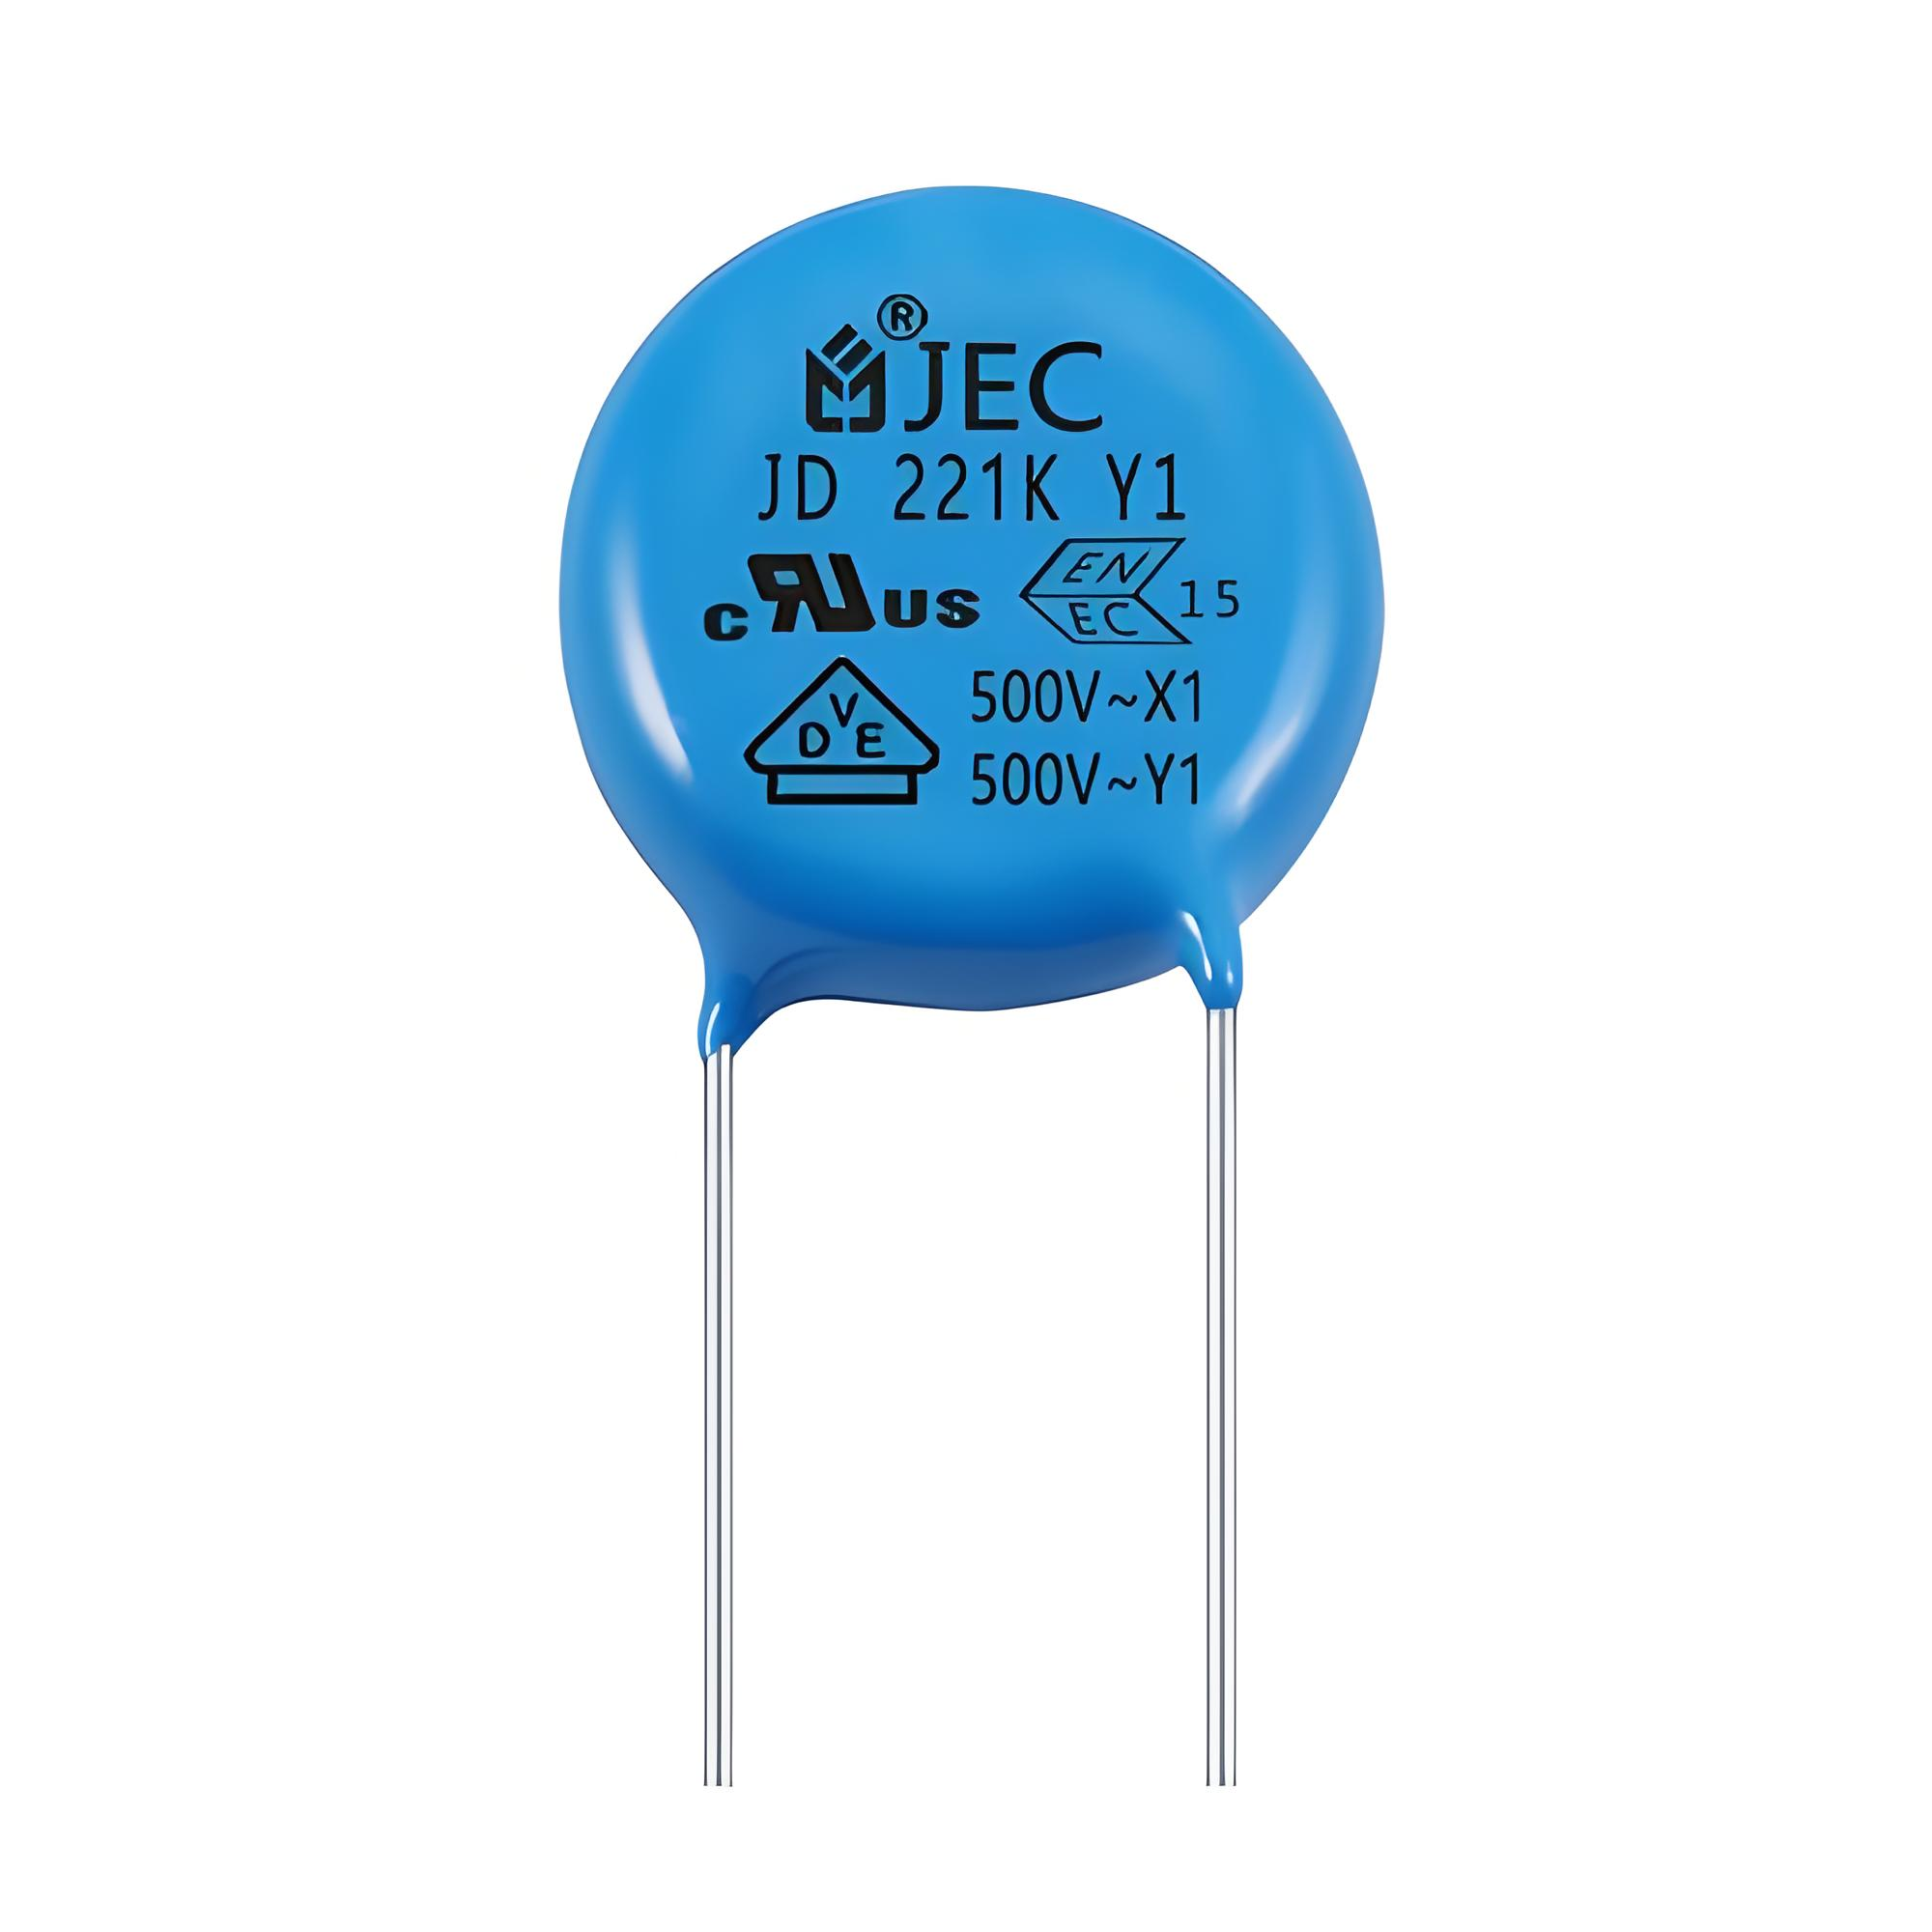
\includegraphics[width=0.6\textwidth]{安规电容Y.jpg}
    \caption{Y电容实物图}
    \label{fig:y_capacitor}
\end{figure}

\paragraph{Y电容的作用}

Y电容的主要作用包括：

\begin{itemize}[leftmargin=2cm]
    \item \textbf{抑制共模干扰}：滤除电源线上的共模噪声
    \item \textbf{安全隔离}：在相线/零线与地线之间提供安全隔离
    \item \textbf{泄放静电}：泄放设备上的静电电荷
    \item \textbf{改善EMC性能}：提高设备的电磁兼容性
    \item \textbf{人身安全保护}：防止触电危险
\end{itemize}

\paragraph{Y电容的分类}

Y电容根据其耐压等级和绝缘等级可分为：

\begin{itemize}[leftmargin=2cm]
    \item \textbf{Y1电容}：双绝缘，耐压 $\ge$ 8 kV，适用于高安全要求
    \item \textbf{Y2电容}：基本绝缘，耐压 $\ge$ 5 kV，最常用的类型
    \item \textbf{Y3电容}：基本绝缘，耐压 $\ge$ 2.5 kV，适用于一般应用
    \item \textbf{Y4电容}：基本绝缘，耐压 $< 2.5$ kV，适用于低电压应用
\end{itemize}

\paragraph{Y电容的特点}

Y电容的主要特点包括：

\begin{itemize}[leftmargin=2cm]
    \item \textbf{容值范围小}：通常为 100 pF $\sim$ 10 nF，以限制漏电流
    \item \textbf{绝缘等级高}：具有高绝缘电阻和绝缘耐压
    \item \textbf{漏电流小}：严格控制漏电流以确保安全
    \item \textbf{温度稳定性好}：在宽温度范围内性能稳定
    \item \textbf{防潮性能好}：具有良好的防潮和耐湿性能
\end{itemize}

\paragraph{Y电容的应用}

Y电容的主要应用场景包括：

\begin{itemize}[leftmargin=2cm]
    \item \textbf{电源输入滤波}：AC-DC电源的输入端
    \item \textbf{开关电源}：各种开关电源的EMI滤波
    \item \textbf{家电设备}：电视机、冰箱、洗衣机、微波炉等
    \item \textbf{工业设备}：工业控制设备、电机驱动等
    \item \textbf{医疗设备}：需要高安全性的医疗电子设备
    \item \textbf{IT设备}：计算机、服务器、网络设备等
\end{itemize}

\paragraph{Y电容的安全要求}

Y电容的安全要求非常严格，主要包括：

\begin{itemize}[leftmargin=2cm]
    \item \textbf{漏电流限制}：漏电流必须小于安全限值（通常 $< 0.75$ mA）
    \item \textbf{绝缘电阻}：绝缘电阻必须足够高（通常 $> 100$ M$\Omega$）
    \item \textbf{耐压测试}：必须通过高电压耐压测试
    \item \textbf{阻燃性}：必须具有良好的阻燃性能
    \item \textbf{双重保护}：通常需要成对使用以提供双重保护
\end{itemize}

\paragraph{Y电容的选择原则}

选择Y电容时应考虑以下因素：

\begin{itemize}[leftmargin=2cm]
    \item \textbf{安全等级}：根据安全要求选择合适的Y等级
    \item \textbf{容值大小}：在满足滤波需求的同时控制漏电流
    \item \textbf{工作电压}：根据电源电压选择合适的耐压
    \item \textbf{温度范围}：根据工作环境选择合适的温度等级
    \item \textbf{安全认证}：确保通过所需的安全认证
    \item \textbf{成对使用}：通常需要在L-PE和N-PE之间成对使用
\end{itemize}

\subsubsection{安规电容的标识}

安规电容的标识通常包括以下信息：

\begin{itemize}[leftmargin=2cm]
    \item \textbf{安全认证标志}：UL、VDE、CSA、CE等认证标志
    \item \textbf{容值}：电容的标称容量
    \item \textbf{耐压}：电容的额定耐压
    \item \textbf{X/Y等级}：X1/X2/X3或Y1/Y2/Y3/Y4
    \item \textbf{温度等级}：工作温度范围
    \item \textbf{生产日期}：制造日期或批号
\end{itemize}

\subsubsection{安规电容的使用注意事项}

使用安规电容时应注意以下事项：

\begin{itemize}[leftmargin=2cm]
    \item \textbf{不要超压使用}：工作电压不得超过额定耐压
    \item \textbf{不要超温使用}：工作温度不得超过额定温度
    \item \textbf{正确连接}：严格按照电路要求连接X电容和Y电容
    \item \textbf{定期检查}：定期检查安规电容的状态
    \item \textbf{及时更换}：发现异常及时更换
    \item \textbf{使用正品}：使用通过安全认证的正品电容
\end{itemize}

\subsubsection{安规电容与普通电容的区别}

安规电容与普通电容的主要区别：

\begin{table}[H]
    \centering
    \begin{tabular}{|c|c|c|}
        \hline
        \textbf{比较项目} & \textbf{安规电容} & \textbf{普通电容} \\
        \hline
        安全认证 & 必须通过安全认证 & 不需要安全认证 \\
        \hline
        耐压等级 & 高，能承受浪涌 & 一般，仅额定电压 \\
        \hline
        阻燃性能 & 良好，不蔓延火焰 & 一般或无要求 \\
        \hline
        可靠性 & 高，长寿命 & 一般 \\
        \hline
        自愈能力 & 通常具有自愈能力 & 一般无自愈能力 \\
        \hline
        漏电流 & Y电容严格限制 & 一般无严格限制 \\
        \hline
        成本 & 较高 & 较低 \\
        \hline
        应用场景 & 安全要求高的场合 & 一般应用 \\
        \hline
    \end{tabular}
    \caption{安规电容与普通电容比较}
    \label{tab:safety_vs_normal_cap}
\end{table}

\subsubsection{安规电容的发展趋势}

安规电容的发展趋势包括：

\begin{itemize}[leftmargin=2cm]
    \item \textbf{小型化}：在保持性能的同时减小体积
    \item \textbf{高容值}：开发更高容值的安规电容
    \item \textbf{耐高温}：提高工作温度范围
    \item \textbf{低损耗}：降低等效串联电阻
    \item \textbf{环保化}：使用环保材料，符合RoHS指令
    \item \textbf{集成化}：与其他元件集成在一起
\end{itemize}

\section{按结构分类}

\subsection{固定电容}

\subsection{可变电容}

\subsection{微调电容}

\section{按极性分类}

\subsection{有极性电容}

\subsection{无极性电容}

\chapter{电容的特性}

\section{电容的电气特性}

\subsection{容值误差}

\subsection{耐压}

\subsection{温度系数}

\subsection{频率特性}

\subsection{等效串联电阻}

\subsection{等效串联电感}

\section{电容的物理特性}

\subsection{尺寸规格}

\subsection{工作温度范围}

\subsection{使用寿命}

\subsection{可靠性}

\chapter{电容在收音机中的应用}

\section{调谐电路}

\subsection{调谐电容}

\subsection{本机振荡电容}

\section{滤波电路}

\subsection{电源滤波电容}

\subsection{信号滤波电容}

\subsection{去耦电容}

\section{耦合电路}

\subsection{信号耦合电容}

\subsection{级间耦合电容}

\section{旁路电路}

\subsection{旁路电容的作用}

\subsection{旁路电容的选择}

\section{振荡电路}

\subsection{RC振荡电路}

\subsection{LC振荡电路}

\chapter{电容的选择原则}

\section{容值选择}

\subsection{根据电路需求选择}

\subsection{标准容值系列}

\section{耐压选择}

\subsection{工作电压与耐压的关系}

\subsection{安全裕量的考虑}

\section{介质选择}

\subsection{不同介质的特点}

\subsection{根据应用场景选择}

\section{精度选择}

\subsection{精度等级}

\subsection{根据精度要求选择}

\section{其他考虑因素}

\subsection{温度系数}

\subsection{尺寸限制}

\subsection{成本因素}

\chapter{电容的规格表示}

\section{容值表示}

\subsection{数值表示法}

\subsection{色环表示法}

\subsection{字母数字表示法}

\section{耐压表示}

\subsection{直接标注法}

\subsection{颜色标注法}

\section{其他标注}

\subsection{温度系数标注}

\subsection{精度标注}

\subsection{极性标注}

\backmatter

\end{document}
